\begin{Figure}[h]
    \centering
    \footnotesize
		
		\psfrag{an}[c][c] {$\text{Solid anode}$}
    \psfrag{ca}[l][l] {$\text{Solid cathode}$}
		\psfrag{fd}[l][c] {$\text{All-solid-state battery}$}
		\psfrag{ch}[l][c] {$\text{Sample: IEK1 - Forschungszentrum Jülich}$}
		
		\psfrag{xx}[c][c] {$\text{Li}+$}
		\psfrag{xxx}[c][c] {$\text{Lithium Lanthanum Zirconate}$}
		\psfrag{em}[c][c] {$\text{e}-$}
		\psfrag{sele}[c][c] {$\text{Solid electrolyte}$}
		\psfrag{gr}[l][c] {$\text{Lithium metal}$}
		\psfrag{mo}[l][c] {$\text{Metal-oxide}$}
		\psfrag{xma}[l][c] {$\text{La}_{7}\text{Li}_{3}\text{Zr}_{2}\text{O}_{12}$}
		
		\psfrag{xbf}[l][c] {$\text{Before}$}
		\psfrag{xat}[l][c] {$\text{After}$}
		
		\psfrag{xm}[c][c] {$-$}
		\psfrag{xp}[c][c] {$+$}
		\psfrag{dta}[c][c] {$\delta x$}
		
		\psfrag{a}[c][c] {$\text{\faBolt}$}
		\psfrag{F}[c][c] {$\text{F}$}
    \includegraphics[width=0.65\textwidth]{dendrite.eps}
    %\caption{Charging mechanism of Li-ion battery cell from a fully-discharged state to a fully-charged state:  $\text{\faBatteryEmpty} \rightarrow \text{\faBatteryFull}$. At current state, Li-ions start moving from cathode to anode.}
    %\label{\LABEL}
		
\end{Figure}


